\chapter{Desenvolvimento do trabalho}

% Apresentar os resultados das fases que transformam
% os requisitos em produtos finais.
% • A estrutura desse capítulo depende do processo de
% desenvolvimento do trabalho.
% • A organização e as seções desse capítulo devem ser
% definidas juntamente com o orientador.

Este capítulo tem como objetivo explicitar quais foram as decisões de projeto que foram tomadas ao longo do desenvolvimento do sistema.

\section{Tecnologias utilizadas}
O projeto pretende definir algumas tecnologias de base para serem usadas durante o desenvolvimento de cada fase dele.

\begin{itemize}
    \item \textbf{Conexão OBD-II:} serão precisos \textit{scanners} automotivos chamados ELM327 \textsuperscript{[14]} para se conectarem aos carros voluntários durante a fase de geração de dados.
    
    \item \textbf{Android Studio:} será a IDE usada para desenvolver o aplicativo que faz a conexão entre o leitor de OBD-II.
    
    \item \textbf{Banco de dados:} deverá ser definido o tipo de banco de dados que será hospedado na infraestrutura de nuvem escolhida; de preferência um com que o grupo já esteja familiarizado.
    
    \item \textbf{\textit{Framework Web}:} para desenvolver o \textit{dashboard} de apresentação de dados será preciso criar uma página Web, por isso será necessário o uso de algum \textit{framework} baseado em \textit{Java Script}, como o \textit{React}, por exemplo, mas isso ainda não foi definido.
    
    \item \textbf{\textit{Python} e plataformas de análise de dados:} servirão de ferramenta para a manipulação dos dados coletados ao fim do projeto.
\end{itemize}
% interface com usuario, banco de dados, conexão obd2

\section{Projeto e implementação}
Esta seção descreverá as decisões feitas durante o trabalho.

Para criar os mapas do aplicativo, foi utilizado o framework Folium. A biblioteca Folium é uma poderosa ferramenta para manipular e visualizar dados geoespaciais usando Python. Com o Folium, é possível criar mapas interativos personalizados e incorporar dados neles de várias maneiras. Para manipular dados usando o Folium, pode-se começar importando a biblioteca e criando um objeto Map que representa o mapa. Em seguida, pode-se adicionar camadas, como marcadores, polígonos e popups, para exibir dados de forma intuitiva no mapa. Além disso, o Folium permite a integração de dados geoespaciais em diferentes formatos, como GeoJSON, tornando-o uma ferramenta flexível para análise e visualização de dados geoespaciais em Python.

Foram utilizadas as seguintes bibliotecas para desenvolver o mapa:
        \begin{center}
         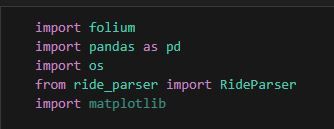
\includegraphics[scale=0.8]         {figures/bibliotecas.JPG}
         \end{center}

A função da classe RideParser é analisar dados dos trajetos.A classe pode receber dados de entrada que descrevem o destino, e então analisa esses dados para extrair informações úteis. Como, por exemplo, traçar a rota feita pelo automóvel. Já o módulo 
''os'' fornece funcionalidades relacionadas ao sistema operacional, permitindo que você interaja com o ambiente do sistema, como manipular diretórios, arquivos, obter informações sobre o sistema, manipular variáveis de ambiente, entre outras tarefas relacionadas ao sistema operacional.
Por fim, tanto a biblioteca pandas, como a matplotlib foram utilizadas para manipular os dados.

Para traçar uma trajetória no mapa usando a biblioteca Folium em Python, será necessário uma lista de pontos de latitude e longitude que representam a trajetória. A partir dos pontos de latitude e longitude colhidos dos sensores do celular, cria-se uma lista de coordenadas que representam os pontos da trajetória. Em seguida, criamos um objeto de mapa usando o Folium e é adicionado uma linha de trajetória (um polilinha) que conecta os pontos da lista e o mapa pode ser visualizado. Uma demonstração de uma trajetória pode ser vista na figura seguinte.

\begin{center}
         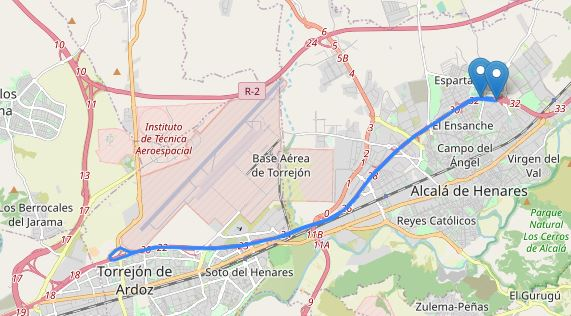
\includegraphics[scale=0.8]         {figures/rota1.JPG}
         \end{center}




\section{Testes e avaliação}
% descrever o plano de testes do sistema: testes de software, modulo, integração e validação
Alguns testes abstratos e macroscópicos podem ser definidos já antes de o projeto começar:

\begin{itemize}
    \item \textbf{Conferir conexão OBD-II:} conectar o dispositivo de leitura na entrada do carro e fazer um \textit{Hello World} através do aplicativo de conexão, mostrando que o protocolo está sendo feito da forma correta.
    
    \item \textbf{Teste de continuidade de transferência de dados:} andar com o carro por alguns minutos e atestar que nenhum dado foi perdido por falta de conexão.
    
    \item \textbf{Equivalência de envio e recepção de dados:} comparar o \textit{log} de envio de dados do aplicativo de interface com a porta OBD-II com o \textit{log} de salvamento do banco de dados hospedado na nuvem; a quantidade de dados, os \textit{timestamps} deles e seus conteúdos devem ser idênticos. 
    
    \item \textbf{Testes de segurança:} de forma bastante ampla, ratificar que não é possível ter acesso aos dados de um certo usuário sem ter as informações de \textit{login}.
    
    \item \textbf{Geração de dados \textit{outliers}:} para verificar se o sistema descarta corretamente as informações que fogem totalmente do padrão esperado ou se consegue pelo menos esconder isso do usuário, para que o \textit{dashboard} mantenha-se com dados consistentes e "limpos", isto é, sem que mostrem números surpreendentes, mas falsos, para o usuário final.
    
\end{itemize}

% Using \texttt{biblatex} you can display a bibliography divided into sections, depending on citation type. 
% Let's cite! Einstein's journal paper \cite{einstein} and Dirac's book \cite{dirac} are physics-related items. 
% Next, \textit{The \LaTeX\ Companion} book \cite{latexcompanion}, Donald Knuth's website \cite{knuthwebsite}, \textit{The Comprehensive Tex Archive Network} (CTAN) \cite{ctan} are \LaTeX-related items; but the others, Donald Knuth's items, \cite{knuth-fa,knuth-acp} are dedicated to programming. 

